%%%%%%%%%%%%%%%%%%%%%%%%%%%%%%%%%%%%%%%%%
% Beamer Presentation
% LaTeX Template
% Version 1.0 (10/11/12)
%
% This template has been downloaded from:
% http://www.LaTeXTemplates.com
%
% License:
% CC BY-NC-SA 3.0 (http://creativecommons.org/licenses/by-nc-sa/3.0/)
%
%%%%%%%%%%%%%%%%%%%%%%%%%%%%%%%%%%%%%%%%%

%----------------------------------------------------------------------------------------
%	PACKAGES AND THEMES
%----------------------------------------------------------------------------------------

\documentclass{beamer}

\mode<presentation> {

% The Beamer class comes with a number of default slide themes
% which change the colors and layouts of slides. Below this is a list
% of all the themes, uncomment each in turn to see what they look like.

%\usetheme{default}
%\usetheme{AnnArbor}
%\usetheme{Antibes}
%\usetheme{Bergen}
%\usetheme{Berkeley}
%\usetheme{Berlin}
%\usetheme{Boadilla}
\usetheme{CambridgeUS}
%\usetheme{Copenhagen}
%\usetheme{Darmstadt}
%\usetheme{Dresden}
%\usetheme{Frankfurt}
%\usetheme{Goettingen}
%\usetheme{Hannover}
%\usetheme{Ilmenau}
%\usetheme{JuanLesPins}
%\usetheme{Luebeck}
%\usetheme{Madrid}
%\usetheme{Malmoe}
%\usetheme{Marburg}
%\usetheme{Montpellier}
%\usetheme{PaloAlto}
%\usetheme{Pittsburgh}
%\usetheme{Rochester}
%\usetheme{Singapore}
%\usetheme{Szeged}
%\usetheme{Warsaw}

% As well as themes, the Beamer class has a number of color themes
% for any slide theme. Uncomment each of these in turn to see how it
% changes the colors of your current slide theme.

%\usecolortheme{albatross}
%\usecolortheme{beaver}
%\usecolortheme{beetle}
%\usecolortheme{crane}
%\usecolortheme{dolphin}
%\usecolortheme{dove}
%\usecolortheme{fly}
%\usecolortheme{lily}
%\usecolortheme{orchid}
%\usecolortheme{rose}
%\usecolortheme{seagull}
\usecolortheme{seahorse}
%\usecolortheme{whale}
%\usecolortheme{wolverine}

%\setbeamertemplate{footline} % To remove the footer line in all slides uncomment this line
%\setbeamertemplate{footline}[page number] % To replace the footer line in all slides with a simple slide count uncomment this line

%\setbeamertemplate{navigation symbols}{} % To remove the navigation symbols from the bottom of all slides uncomment this line
}

\usepackage{graphicx} % Allows including images
\usepackage{booktabs} % Allows the use of \toprule, \midrule and \bottomrule in tables
\usepackage{amsmath}
\usepackage{mathtools}

%----------------------------------------------------------------------------------------
%	TITLE PAGE
%----------------------------------------------------------------------------------------

\title[Online Decision-making]{Online Decision-making with a Expert Committee and Its Application on FahsionFlow} % The short title appears at the bottom of every slide, the full title is only on the title page

\author{Zalando Search Team} % Your name
\institute[Zalando SE] % Your institution as it will appear on the bottom of every slide, may be shorthand to save space
{
Zalando SE \\ % Your institution for the title page
\medskip
\textit{hanchen.xiong@zalando.de} % Your email address
}
\date{\today} % Date, can be changed to a custom date

\begin{document}

\begin{frame}
\titlepage % Print the title page as the first slide
\end{frame}

\begin{frame}
\frametitle{Overview} % Table of contents slide, comment this block out to remove it
\tableofcontents % Throughout your presentation, if you choose to use \section{} and \subsection{} commands, these will automatically be printed on this slide as an overview of your presentation
\end{frame}

%----------------------------------------------------------------------------------------
%	PRESENTATION SLIDES
%----------------------------------------------------------------------------------------

%------------------------------------------------
\section[Online prediction with experts, games, convex optimization]{Online prediction with experts,repeated game playing and convex optimization}        % Sections can be created in order to organize your presentation into discrete blocks, all sections and subsections are automatically printed in the table of contents as an overview of the talk
\frame{
    \frametitle{}
    \Huge{Online prediction with experts, repeated game playing and convex optimization}
}

\subsection{Prediction with Experts' advice}
\frame{
    \frametitle{A gentle start} 
    \begin{itemize}
    \item<1->  \structure{Task:}  online prediction of a binary sequence, \emph{i.e.} sequentially forecast a value $y^{(t)}\in\{-1,1\}$ at time $t$ based on historical values $\{y^{(i)}\}_{i=1}^t$;
    \item<2->  \structure{Expert committee:} an expert $E_{n}$ is a man/woman who can make a prediction, $f_{n}^{(t)}$, using different strategies (algorithms/heuristics/data resources); assume there are $N$ experts in the committee; 
    \item<3->  \structure{Side information:} other task-relevant information may available, \emph{e.g.} $\{\mathbf{x}^{(t)}\}_{i=1}^{t}$;
    \item<4->  \structure{Forecaster: } an aggregating policy $\pi$ is a function which map experts' advices $\Longrightarrow$ final decision $\hat{y}_t$: $\hat{y}_t = \pi(f_{1}^{(t)}, f_{2}^{(t)}, \cdots, f_{N}^{(t)})$; 
    \item<5->  \structure{Weights update:} at the beginning, each expert is assigned a (uniform) weight $w_{n,0}=1$, and it will be updated along the sequence; 
    \item<6->  \structure{Loss:}  $l(\hat{y}^{(t)}, y^{(t)}) = \mathbf{1}_{\hat{y}^{(t)} \neq y^{(t)}}$, $l(f_{n}^{(t)}, y^{(t)}) = \mathbf{1}_{f_{n}^{(t)} \neq y^{(t)}}$
    \end{itemize}
}


\frame{
    \frametitle{A gentle start, cont.} 
    \onslide<+->{\begin{block}{A simple policy}
    The final decision is made with the \alert{majority voting} from the expert committee: $\hat{y}^{(t)} = \textbf{sign} (\frac{\sum_{n=1}^N f_{i}^{(t)}}{N} - 0.5 )$;
    \end{block}}
    
    \onslide<+->{\begin{block}{A simple weight update scheme}
    $w_{n}^{(t)} \leftarrow 0$ if expert $E_{n}$ makes a mistake at time $t-1$, \emph{i.e.} kick $E_n$ out of the committee; 
    \end{block}}

    \onslide<+->{\begin{block}{An ideal scenario}
    we know that there exist some experts who are perfect in the given task;  
    \end{block}}

    \onslide<+->{
    \textbf{Cummulative loss}:
    \begin{equation}
     \hat{L}^{(t)} = \sum_{i=t}^{t}l(\hat{y}^{(t)}, y^{(t)}) \leq \log_{2}N; 
    \end{equation}
    }
}

\frame{
    \frametitle{Generalized committee}
    \onslide<+->{\begin{block}{A more realistic scenario}
     we know that in the committee there exists a best expert who can work better than others in the given task;
    \end{block}}
    \onslide<+->{
    \textbf{Regret $R_{n}^{(t)}$}: the extra losses the forecaster made without exclusively following the expert $E_n$  up to time $t$: 
    \begin{equation}
     R_{n}^{(t)}= \hat{L}^{(t)} - L_{n}^{(t)} = \sum_{i=t}^{t}l(\hat{y}^{(t)}, y^{(t)}) - \sum_{i=t}^{t}l(f_{n}^{(t)}, y^{(t)})
    \end{equation}
    }

    \onslide<+->{\begin{block}{the upper bound of regret}
    $R^{(t)*} = \max_{n\in[1,N]} R_{n}^{(t)} = \hat{L}^{(t)} - \min_{n\in[1,N]}L_{n}^{(t)}$
    \end{block}}
}
    

\frame{
    \frametitle{Weighted majority algorithm}
    \begin{itemize}
    \item  \structure{Task:}  online prediction of a binary sequence, \emph{i.e.} sequentially forecast a value $y^{(t)}\in\{-1,1\}$ at time $t$ based on historical values $\{y^{(i)}\}_{i=1}^t$;
    \item  \structure{Expert committee:} an expert $E_{n}$ is a man/woman who can make a prediction, $f_{n}^{(t)}$, using different strategies (algorithms/heuristics/data resources); assume there are $N$ experts in the committee; 
    \item  \structure{Loss:}  $l(\hat{y}^{(t)}, y^{(t)}) = \mathbf{1}_{\hat{y}^{(t)} \neq y^{(t)}}$, $l(f_{n}^{(t)}, y^{(t)}) = \mathbf{1}_{f_{n}^{(t)} \neq y^{(t)}}$
    \line(1,0){450} 
    \item <2->  \alert{Forecaster: }  $\hat{y}_t = \textbf{sign}(\sum_{n:f_{n,t} =1}w_n^{(t-1)} - \sum_{m:f_{m,t} =-1}w_m^{(t-1)} )$;
    \item <3->  \alert{Weights update:} if one expert $E_n$ predicts wrongly, decrease its weight 
    \begin{equation}
       w_{n}^{(t+1)} = (1-\eta) w_n^{(t)}  
    \end{equation}
    where $\eta \leq \frac{1}{2}$. 
    \end{itemize}   
}


\frame{
    \frametitle{Analysis on weighted majority algorithm}
    \onslide<+->{
    \begin{theorem}[cummulative loss bound using weighted majority]
    After T steps, $\hat{L}^{(T)} \leq 2(1+\eta) \min_{1\in[1,N]} L_{n}^{(T)} + \frac{2\ln N}{\eta}$
    \end{theorem}
    }
    \onslide<+->{
    \alert{Proof:}  Let $\Gamma^{(t)} = \sum_{n \in [1,N]} w_n^{(t)}$, then $\Gamma^{(1)}= N$. Also, if the forecaster makes 
    a mistake, $\hat{y}^{(t)} \neq y^{(t)}$ 
    \begin{equation}
      \Gamma^{(t+1)} \leq \Gamma^{(t)} (\frac{1}{2} + \frac{1}{2} (1-\eta) = \Gamma^{(t)} (1- \frac{\eta}{2})
    \end{equation}
    therefore: 
    \begin{equation}
       \Gamma^{(T+1)} \leq N (1-\frac{\eta}{2})^{\hat{L}^{(T)}} 
    \end{equation}
    for any individual expert $n$
    \begin{equation}
       w_n^{(T+1)}  = (1-\eta)^{L_n^{(T)}}
    \end{equation}
    since $w_n^{(T+1)} \leq \Gamma^{(T+1)} \Longrightarrow(1-\eta)^{L_n^{(T)}} \leq N (1-\frac{\eta}{2})^{\hat{L}^{(T)}} $
    }  
}

\frame{
    \frametitle{Analysis on weighted majority algorithm, cont.}
    \begin{equation}
    \begin{array}{rcl}
                        (1-\eta)^{L_n^{(T)}}    & \leq &  N (1-\frac{\eta}{2})^{\hat{L}^{(T)}}  \\ \\
    \Leftrightarrow         L_n^{(T)} \ln (1-\eta)  & \leq &  \ln N +  \hat{L}^{(T)}  \ln (1-\frac{\eta}{2}) \\ \\
    \Leftrightarrow       -\ln (1-\frac{\eta}{2})   & \leq &  -L_n^{(T)} \ln (1-\eta) + \ln N  \\ \\  
    \xRightarrow{\alert{x\leq -\ln (1-x)}}  \frac{\eta}{2} \hat{L}^{(T)} & \leq & -L_n^{(T)} \ln (1-\eta) + \ln N  \\ \\  
    \xRightarrow{\alert{-\ln (1-x) \leq x + x^2, \text{when } x \leq 1/2 }}  \frac{\eta}{2}  \hat{L}^{(T)} & \leq & L_n^{(T)} \eta(1+\eta) + \ln N  \\ \\  
    \Leftrightarrow  \hat{L}^{(T)} & \leq & 2(1+\eta) L_{n}^{(T)} + \frac{2\ln N}{\eta}
    \end{array}
    \end{equation} 
}

\frame{
    \frametitle{Randomized weighted majority algorithm}
    \begin{itemize}
    \item  \structure{Task:}  online prediction of a binary sequence, \emph{i.e.} sequentially forecast a value $y^{(t)}\in\{-1,1\}$ at time $t$ based on historical values $\{y^{(i)}\}_{i=1}^t$;
    \item  \structure{Expert committee:} an expert $E_{n}$ is a man/woman who can make a prediction, $f_{n}^{(t)}$, using different strategies (algorithms/heuristics/data resources); assume there are $N$ experts in the committee; 
    \item  \structure{Loss:}  $l(\hat{y}^{(t)}, y^{(t)}) = \mathbf{1}_{\hat{y}^{(t)} \neq y^{(t)}}$, $l(f_{n}^{(t)}, y^{(t)}) = \mathbf{1}_{f_{n}^{(t)} \neq y^{(t)}}$
    \item  \structure{Weights update:} if one expert $E_n$ predicts wrongly, decrease its weight 
    \begin{equation}
       w_{n}^{(t+1)} = (1-\eta) w_n^{(t)}  
    \end{equation}
    where $\eta \leq 1/2$. 
    \line(1,0){450} 
    \item <2->  \alert{Forecaster: }  $\hat{y}_t \sim  \textbf{Bernoulli}\left(\frac{\sum_{n:f_{n,t} =1} w_n^{(t-1)}}{\sum_n w_n^{(t-1)}}, \frac{\sum_{n:f_{n,t} =-1} w_n^{(t-1)}}{\sum_n w_n^{(t-1)}}\right)$;
    \end{itemize}   
}

\frame{
    \frametitle{Analysis on randomized weighted majority algorithm}
    \onslide<+->{
    \begin{theorem}[cummulative loss bound using randomized weighted majority]
    After T steps, $\hat{L}^{(T)} \leq (1+\eta) \min_{1\in[1,N]} L_{n}^{(T)} + \frac{\ln N}{\eta}$
    \end{theorem}
    }
    \onslide<+->{
    \alert{Proof:}  Let $\Gamma^{(t)} = \sum_{n \in [1,N]} w_n^{(t)}$, then $\Gamma^{(1)}= N$. 
    \newline 
    At each time $t$, let $F^(t) = \frac{\sum_{n:f_n^{(t)} \neq y^{(t)}} w^{(t)}_n }{\sum_{n} w_n^{(t)}}$, then 
    \begin{equation}
      \Gamma^{(t+1)} = \Gamma^{(t)} \Big( 1-F^{(t)} + F^{(t)}(1-\eta) \Big) = \Gamma^{(t)} (1- F^{(t)}\eta)
    \end{equation}
    therefore: 
    \begin{equation}
       \Gamma^{(T+1)} = N \prod_{t=1}^T(1-F^{(t)}\eta) 
    \end{equation}
    for any individual expert $n:       w_n^{(T+1)}  = (1-\eta)^{L_n^{(T)}}$, \\
    since $w_n^{(T+1)} \leq \Gamma^{(T+1)} \Longrightarrow(1-\eta)^{L_n^{(T)}} \leq N \prod_{t=1}^T(1-F^{(t)}\eta)$
    }  
}


\frame{
    \frametitle{Go beyond binary sequence and 0-1 loss}
    \begin{itemize} 
    \item  \structure{Expert committee:} an expert $E_{n}$ is a man/woman who can make a prediction, $f_{n}^{(t)}$, using different strategies (algorithms/heuristics/data resources); assume there are $N$ experts in the committee; 
    \item  \structure{Forecaster: }  $\hat{y}^{(t)} = \pi(f_{1}^{(t)}, f_{2}^{(t)}, \cdots, f_{N}^{(t)})$; 
    \line(1,0){450} 
    \item  \alert{Task:}  \alert{general online prediction}, \emph{i.e.} sequentially forecast a value $y^{(t)}\in\mathbb{R}$ at time $t$ based on historical values $\{y^{(i)}\}_{i=1}^t$;
    \item  \alert{Loss:}  a cost vector $[m_1^{(t)}, m_2^{(t)}i, \cdots, m_N^{(t)}]$ is incurred to experts' predictions at time $t$;
    \item  \alert{Weights update:}  multiplicative manner
    \begin{equation}
        w_n^{(t+1)} = w_n^{(t)} g(m_n^{(t)})
    \end{equation}
    where $g(x)$ is a decreasing function w.r.t. $x$. 
    \end{itemize}   
}

\frame{
    \frametitle{Revisit aggregation policy in binary case}
     \alert{Forecaster: }  $\hat{y}_t \sim  \textbf{Bernoulli}\left(\frac{\sum_{n:f_{n,t} =1} w_n^{(t-1)}}{\sum_n w_n^{(t-1)}}, \frac{\sum_{n:f_{n,t} =-1} w_n^{(t-1)}}{\sum_n w_n^{(t-1)}}\right)$;
     \newline 
     Let $p^{(t-1)}_n = \frac{w_n^{(t-1)}}{\sum_{n=1}^N w_n^{(t-1)}}$, then 
     \begin{equation}
     \begin{array}{rcl}
        \mathbb{E}\left\{ \hat{y}^{(t)}\right\} & = & (-1)\cdot \sum_{n:f_{n,t}=-1} p_n^{(t-1)}  + 1 \cdot \sum_{n:f_{n,t}=1} p_n^{(t-1)}  \\ \\
                                                & = &  \sum_{n=1} f_n^{(t)} p_n^{(t-1)} \\   \\
                                                & = &  \mathbb{E}_{p^{(t-1)}} \left\{ f^{(t)} \right\}
    \end{array}
     \end{equation}
     A further randomized version:  
     \begin{equation}
         \hat{y}^{(t)} = f_{n_\dagger}^{(t)} \text{ with } n_\dagger \sim [p_1^{(t-1)},  p_2^{(t-1)}, \cdots,p_N^{(t-1)}]
     \end{equation}  
}

\frame{
    \frametitle{Randomized weighted majority algorithm IN GENERAL}
    \begin{itemize} 
    \item  \structure{Expert committee:} an expert $E_{n}$ is a man/woman who can make a prediction, $f_{n}^{(t)}$, using different strategies (algorithms/heuristics/data resources); assume there are $N$ experts in the committee; 
    \line(1,0){450} 
    \item  \alert{Task:}  \alert{general online prediction}, \emph{i.e.} sequentially forecast a value $y^{(t)}\in\mathbb{R}$ at time $t$ based on historical values $\{y^{(i)}\}_{i=1}^t$;
    \item  \alert{Loss:}  a cost vector $[m_1^{(t)}, m_2^{(t)}i, \cdots, m_N^{(t)}]$ is incurred to experts' predictions at time $t$;
    \item  \alert{Forecaster: } $\hat{y}^{(t)} = f_{n_\dagger}^{(t)} \text{ with } n_\dagger \sim [p_1^{(t-1)},  p_2^{(t-1)}, \cdots,p_N^{(t-1)}]$ 
    \item  \alert{Weights update:}  multiplicative manner
    \begin{equation}
        w_n^{(t+1)} = w_n^{(t)}(1-\eta m_n^{(t)})
    \end{equation}
    where $\eta \leq 1/2$
    \end{itemize}   
}

\frame{
    \frametitle{Analysis} 
    \begin{theorem}[Regret bound using randomized weighted majority]
    When $m_n^{(t)} \in [-1, 1], \forall n,t$, after T steps,  \newline
    $\hat{L}^{(T)} \leq \min_{1\in[1,N]} L_{n}^{(T)} + \eta \sum_{t=1}^T |m_n^{(t)}|_1 + \frac{\ln N}{\eta}$
    \end{theorem}
    \alert{Regret bound }: $\mathbf{R}^* \leq \eta T + \frac{\ln N}{\eta}$
}

\frame{
    \frametitle{Hedge algorithm}
    \begin{block}{}
    \alert{Weights update:} 
    \begin{equation}
        w_n^{(t+1)} = w_n^{(t)} \exp(-\eta m_n^{(t)})
    \end{equation}
    where $\eta \in[0,1]$.
    \end{block}
    \begin{theorem}[Regret bound using randomized weighted majority]
    When $m_n^{(t)} \in [-1, 1], \forall n,t$, after T steps,  \newline
    $\hat{L}^{(T)} \leq \min_{1\in[1,N]} L_{n}^{(T)} + \eta \sum_{t=1}^T |m_n^{(t)}|_1 + \frac{\ln N}{\eta}$
    \end{theorem}  
}


\subsection{Online repeated game playing}
\frame{
 \frametitle{One-player game}
 \begin{itemize}
 \item<1-> One player plays a game, at time $t$ he takes one action $a^{(t)} = i\in[1,N]$, then the environment 
 releases the cost for each action $\mathbf{m}^{(t)} = [m_1^{(t)}, m_2^{(t)},\cdots, m_N^{(t)}]^\top, m_n^{(t)}\in[-1,1]$,
 \item<1-> \alert{Note} that the loss function $\mathbf{m}^{(t)}$ can change over time, i.e. the environment is changing.
 \item<2-> if the player selects actions by the probabilities $\mathbf{p}^{(t)}$ computed by randomized weighted majority and update them accordingly, then 
 \begin{equation}
    \sum_{t=1}^T \langle \mathbf{m}^{(t)}, \mathbf{p}^{(t)}\rangle \leq  \sum_{t=1}^T m_i^{(t)} + \eta T + \frac{\ln n}{\eta}
 \end{equation}
 \end{itemize}
}

\frame{
\frametitle{Two-player game} 
\alert{Two-person zero-sum}: two players ($K=2)$ play a game which is defined by a $N\times N$ cost matrix $\mathbf{C}$ ($N$ is 
the number of possible actions for players) , where 
each entry $c_{ij}$ defines \alert{the loss to the row player} when the \structure{row player} takes the action $i\in [1,N]$ and 
the \structure{column player} takes the action $j\in [1,N]$. 


An example cost matrix: 
$\left[\begin{array}{ccccc}
  &   1         &   2         &   3         &   4   \\
1 &   c_{11}    &   c_{12}    &   c_{13}    &   c_{14} \\
2 &   c_{21}    &   c_{22}    &   c_{23}    &   c_{24} \\
3 &   c_{31}    &   c_{32}    &   c_{33}    &   c_{34} \\
4 &   c_{41}    &   c_{42}    &   c_{43}    &   c_{44} 
\end{array}
\right]$

The row player's goal is to minimize its loss while the objective of the column player is to maximize it 

}

\frame{
    \frametitle{Nash Equilibrium}
    \begin{itemize}
      \item<1-> no player has an incentive of changing his strategy if the player does not change his, i.e. every player is happy about 
      current status; 
      \item<2-> 
    \end{itemize}
}


\frame{
    \frametitle{Hanan's algorithm for two-player zero-sum game}
    \begin{block}{Follow the perturbed leading expert}
     \alert{Forecaster:}  select the action  $i^{(t)} = \arg\min_{i\in [1,N]} \left\{L_i^{(t-1)} + \tau_i \right\}$ 
     where $\tau_i$ are randomly sampled from $[0, 1/\epsilon]$
    \end{block}
}



\subsection{Online convex optimization}
\frame{
    \frametitle{Arbitrary convex loss function}
}


\frame{
    \frametitle{Portfolio management}
    $f_t{i} = \log (-\langle \mathbf{p}_i, \Delta x_{t} \rangle)$
}


\frame{
    \frametitle{Adaboost}
}



%-----------------------------------------------------------------------------------------
\section{Bandit Optimization in metric spaces}
\frame{
    \frametitle{}
    \Huge{Bandit Optimization in metric spaces}
}
\subsection{Bandit: play games with limited feedbacks}
\frame{
    \frametitle{Observe only one cost}  
     \begin{itemize}
        \item  <1-> One player plays a game, at time $t$ he takes one action $a^{(t)} = i\in[1,N]$, then the environment 
            releases the cost for \alert{only the selected action} $m_{a^{(t)}}^{(t)}$, 
        \item  <2-> playing games in a Bandit setting falls into  \alert{classic exploitation v.s. exploration dilemma} 
 \end{itemize}
}


\frame{
    \frametitle{Multi-armed bandit problem}
    \begin{figure}     
        
\includegraphics[width = 0.5\textwidth]{bandit-arm}
    \end{figure}
}

\frame{
    \frametitle{Upper confidence bound}
    \begin{itemize}
     \item <1-> at each time $t$, play the arm $i^{(t)}$ by 
     \begin{equation}
        i^{(t)} = \arg\max_{i\in [1,N]} \left\{\textbf{avg.} [m_i] + \sqrt{\frac{2\ln t}{T_i}} \right\}
     \end{equation}
     \item <2-> Regret bound:
     \begin{equation}
       \mathbf{R}^{(t)*} \leq \left[ 8 \sum_{i: \mu_i < \mu^* }\frac{\ln t}{\mu^* -\mu_i } \right] + (1+\frac{\pi^2}{3}) (\sum_{i=1}^N (\mu^*-\mu_i) )
     \end{equation}
     where $\mu_i$ denote the true expected reward for arm $i$, and $\mu^*$ denote the best one.
    \end{itemize}
}


\subsection{Gaussian process bandit optimization}
\frame{
    \frametitle{Contextual bandit optimization}
    \begin{itemize}
       \item <1-> in classic multi-armed bandit problem, all arms are \alert{independent};   
       \item <2-> in many practical applications, \alert{there exist context beneath arms}, e.g. \structure{representation of arms is in a metric space};    
    \end{itemize}
}

\frame{
    \frametitle{Response surface optimization}
    \begin{itemize}
       \item <1->  response surface optimization is an extension of contextual bandit optimization to infinite number of arms; 
       \item <2->  model the response of arms using a smooth surface function $f$ 
       \item <3-> a demo mimicking Fashionflow style to understand surface-response optimization; 
       \item <4-> a most general case, \alert{Lipschit  continuity}: if 
       \begin{equation}
            d_x(\mathbf{x}_1, \mathbf{x}_2) \leq L \cdot d_f(f(\mathbf{x}_1), f(\mathbf{x}_2))
       \end{equation}
       then we say $f$ is a $L$-Lipschit continuous function. 
    \end{itemize}
}

\frame{
    \frametitle{Gaussian process}
    \onslide<+->\begin{block}{Definition}
    A Gaussian process (GP) defines is a collection of random variables, any finite number of of which have joint Gaussian distribution.
     \begin{equation}
          f(\mathbf{x}) \sim \mathcal{GP} (\mu(\mathbf{x}), k(\mathbf{x},\mathbf{x}^\prime))
     \end{equation}
    \end{block}
    \onslide<+->\begin{block}{joint Gaussian distribution}
    \begin{equation}
        \left[
        \begin{array}{c}
        f(\mathbf{X}_{train}) \\
        f(\mathbf{x}_{test})
        \end{array}
        \right]
        \sim  \left(
        \left[ 
        \begin{array}{c}
        \mu(\mathbf{X}_{train}) \\
        \mu(\mathbf{x}_{test}) 
        \end{array}
        \right], 
        \left[
           \begin{array}{cc}
             k(X_{train}, X_{train})              , &  k(\mathbf{X}_{train}, \mathbf{x}_{test})  \\
             k(\mathbf{X}_{train}, x_{test})^\top , &  k(\mathbf{x}_{test}, \mathbf{x}_{test})
           \end{array}
        \right]
        \right)
    \end{equation}
    \end{block}
}
\frame{
  \frametitle{Gaussian process, cont.}
    \onslide<+-> \begin{block} {Conditional probability}
    \begin{equation}
         f(\mathbf{x}_{test})| f(\mathbf{X}_{train}) \sim  \mathcal{N} \left(\mu_{pos}(\mathbf{x}_{test}), k_{pos}(\mathbf{x}_{test}, \mathbf{x}^{\prime}) \right)
    \end{equation} 
    \end{block}
   \onslide<+-> \begin{block}{Posterior Gaussian process}
        \begin{equation}
         f(\mathbf{x})|\mathcal{D}_{train} \sim \mathcal{GP} \left(\mu_{pos}(\mathbf{x}), k_{pos}(\mathbf{x}, \mathbf{x}^\prime)\right)
    \end{equation}
    \end{block}
    where  $\mu_{pos}(\mathbf{x}) = \mu(\mathbf{x}) + k(\mathbf{X}_{train}, \mathbf{x})^\top  k(X_{train}, X_{train}) (f(\mathbf{X}_{train}) - \mathbf{X}_{train}) $ and 
    $k_{pos}(\mathbf{x}, \mathbf{x}^\prime) = k(\mathbf{x}, \mathbf{x}^\prime) - k(\mathbf{X}_{train}, \mathbf{x})^\top k(\mathbf{X}_{train}, \mathbf{X}_{train})^{-1} k(\mathbf{X}_{train}, \mathbf{x}^\prime) $.
}


\frame{
    \frametitle{Gaussian process bandit optimization}
    \begin{block}{Kernel function}
       squared exponential kernel:  $k(\mathbf{x}, \mathbf{x}^\prime) = \exp(-\frac{||\mathbf{x} - \mathbf{x}^\prime||}{2l^2})$
    \end{block}
    \begin{block}{Information gain} 
        the informativeness of  a set of points  $A \in \mathcal{X}$ for learning $f$ is defined as:
        \begin{equation}
         I(\mathbf{y}_A; \mathbf{f}_A) = H(\mathbf{y}_A) - H(\mathbf{y}_A|\mathbf{f}_A)
        \end{equation}
    \end{block}
    \begin{block}{Maximum information gain after $T$ iterations} 
      $\gamma^{(T)} = \max_{A\in \mathcal{X}:|A|=T}  I(\mathbf{y}_A; \mathbf{f}_A)$
    \end{block}

}

\frame{
    \frametitle{Upper confidence bound}
    \begin{itemize}
      \item <1-> at each time $t$, chose: 
     \begin{equation}
        \mathbf{x}^{(t)} = \arg\max_{\mathbf{x} \in \mathcal{X}} \mu^{(t-1)}(\mathbf{x}) + \kappa^{(t)} \sigma^{(t-1)}(\mathbf{x})
     \end{equation}
     where $\kappa^{(t)} = 2B + 300 \gamma^{(t)} \log^3(t/\delta)$, $||f||^2 \leq B$ 
     \item <2-> Regret bound:
     \begin{equation}
          Pr\left\{\mathbf{R}^{(T)*} \leq \sqrt{\frac{8}{\log(1+\sigma^{-1})} T \beta^{(T)}\gamma^{(T)}}\right\} \geq 1-\delta
     \end{equation}
    \end{itemize}
}

\subsection{General Bayesian optimization} 
\frame{
    \frametitle{Regression with ensemble models}
    \begin{itemize} 
       \item <1->  Gaussian process bandit optimization is an instance of Bayesian optimization; 
       \item <1->  any function $f$ with certain \structure{smoothness assumption} and \structure{uncertainty measurement} can be used as a pseudo Bayesian optimization;
       \item <2->  \alert{one example:}  an ensemble of linear functions
       \begin{enumerate}
        \item \structure{smoothness assumption}: average of linear functions
        \begin{figure}
            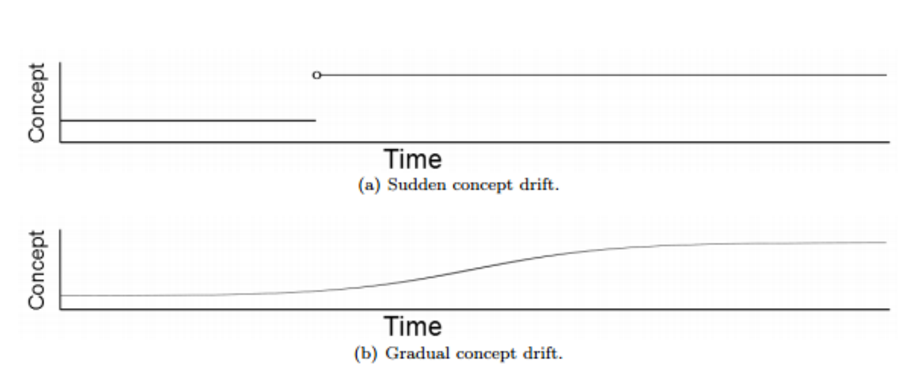
\includegraphics[width = 0.3\textwidth] {concept_drift}
        \end{figure}
        \item \structure{uncertainty measurement}: std.of linear functions 
       \end{enumerate}
       \item <2->  advantage: can better exploit task-relevant features instead of \alert{isotropic length-scale} in kernel function 
    \end{itemize}
}

%------------------------------------------------------------------------------------------
\section{Concept drift in online decision}
\frame{
    \frametitle{}
    \Huge{Concept drift in online decision}
}
\frame{
    \frametitle{What do people do when the concept drifts ?}
    \begin{figure}
     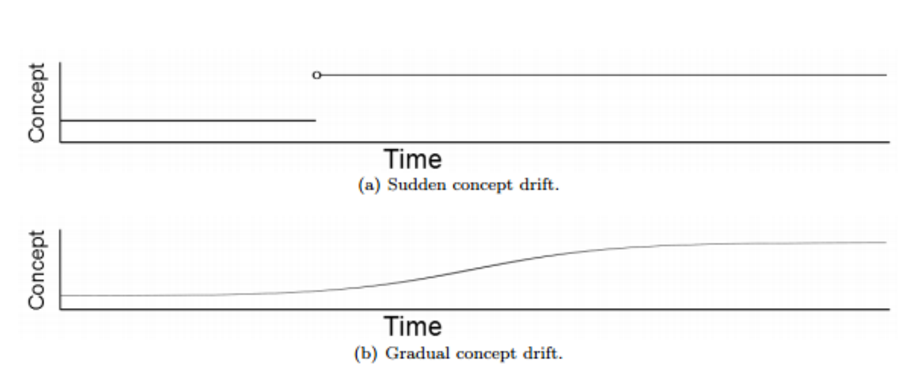
\includegraphics[width = 0.7\textwidth]{concept_drift}
    \end{figure}
   Assume that the concept drift can be successfully detected, 
    \begin{itemize}
       \item <1-> \structure{forget the data} before the new concept in learning algorithms; 
       \item <2-> \alert{change a new learning algorithm (strategy))}
    \end{itemize}
}
\subsection{Stability v.s. adaptivity}
\frame{
    \frametitle{Stability and adaptivity when forgetting data}
    \begin{block}{Definition} 
        A learning algorithm $\mathcal{A}$ has error stability $\beta_n$ with respect to the loss function $l$ if 
        \begin{equation*}
            \forall Z_n \in \mathcal{X}^n, \forall i\in \{1,\cdots, n\} |\mathbb{E}\{l(\mathcal{A}_{Z_n})\} - \mathbb{E}\{l(\mathcal{A}_{Z_n}^{-i})\} | 
        \end{equation*}
    \end{block}
    \begin{block}{Examples}
        for k-NN, SVM, support vector regression and ridge regression, $\beta_n = \mathcal{O}(\frac{1}{n{)$
    \end{block}
    
}
\subsection{Explicit detection of concept drifts}
\frame{
    \frametitle{Detect concept drift}
}
\subsection{Adaptive regret for tracking the best expert}
\frame{
    \frametitle{Concept drift = the best expert shift}
}
\subsection{Time-varying surface-response bandit optimization}
\frame{
    \frametitle{Temporal-spatial kernel}
}



%------------------------------------------------------------------------------------------
\section{Sku Proposal in FashionFlow}
\subsection{Expert setting v.s. Bandit setting}
\frame{
    \frametitle{Expert committee setting}
    
}

\frame{
    \frametitle{Bandit setting}
}


\subsection{Algorithm evaluation}

%------------------------------------------------

\begin{frame}
\Huge{\centerline{The End}}
\end{frame}

%----------------------------------------------------------------------------------------

\end{document} 
